\section{Теория.}

Движение электронов в электрических и магнитных поля описывается уравнением:

$ \frac{d^2 \overline{r}}{dt^2} = \frac{e}{m} \left ( \overline(E) + \left [ \frac{d \overline{r}}{dt} \right ] \right )$

где $\overline{r}$ "--- радиус"=ектор электрона $e$ "--- заряд электрона, $m$ "--- масса электрона, $\overline{E}$ "--- вектор напряженности электрического поля; $\overline{B}$ "--- вектор индукции магнитного поля.

Видно, что движение электрона определяется конфигурацией поля и отношением заряда электрона к его массе. Отсюда следует важность и необходимасть определения величины $\frac{e}{m}$, называемой удельным зарядом электрона.

В настоящей лабораторной работе поставлена задача найти отношение заряда электрона к его массе. Для этой цели используется цилиндрический диод, помещенный в солеонид, который создает аксиальное магнитное поле. Направление вектора магнитной индукции совпадает с осью симметрии лампы. В области движения электронов, имитируетмых катодом, реализуются скрещенные электрическое и магнитное поля. Такая конфигурация электрического и магнитмного полей характерна для магнетронов "--- генераторов электромагнитных колебаний сверхвысоких частот. Поэтому описываемый метод измерения величины $\frac{e}{m}$ и получил название <<метода магнетрона>>. Как было показано в разделе <<Общие теоретические замечания>>, под действием магнитного поля траектории электронов в диоде становятся криволинейными. При критической величине индукции магнитного поля, определяемой формуллой

\begin{equation}
    B_k = \frac{2}{r_a} \cdot \sqrt[2]{\frac{2 V_a}{\frac{e}{m}}}
    \label{eq:formula1}
\end{equation}

электроны перестают достигать андоа. При этом электроны образуют отрицательный пространственный заряд, который движется в пространстве между катодом и анодом, но сила анодного тока равна нулю.

Из \ref{eq:formula1} следует

\begin{equation}
    \frac{e}{m} = \frac{8 V_a}{r^2_a B^2_k}
    \label{eq:formula2}
\end{equation}

Напомним, что соотношение (\ref{eq:formula1}), а следовательно и (\ref{eq:formula2}), справедливы в том случае, когда радиус катода значительно меньше радиуса анода. По формуле (\ref{eq:formula2}) и найденным из опыта значениям $V_a$ и $В_k$ в настоящей лабораторной работе определяется величина $\frac{e}{m}$. Если индукцию магнитного поля, в котором находится диод, постепенно увеличивать, то критическое состояние ($В = В_k$) можно обнаружить по спаду тока, идущего через диод.

На рис. 1 приведена статическая характеристика, дающая зависимость величины тока через диод $I_a$ от силы тока $I_c$ в соленоиде, создающего магнитное поле (при $V_a = const$). Поскольку индукция магнитного поля В внутри соленоида линейно зависит от силы тока $I_c$, то этот график фактически представляет собой зависимость $I_a$ от $B$. Первоначальное увеличение тока через соленоид (увеличение $B$) практически не вызывает изменения анодного тока, так как в этих условиях подавляющее число электронов, движущихся от катода, попадает на анод. Когда величина $I_c$ приближается к критическому значению, происходит резкое уменьшение анодного тока. Если бы все электроны у поверхности катода имели одинаковые скорости, то кривая, характеризующая зависимость $I_a = f(I_c)$, спадала бы вертикально вниз. Фактически имеется лишь довольно крутой спад этой кривой, что связано с разбросом по скоростям термоэмиссионных электронов (критические условия достигаются для различных электронов при разных значениях $B$ или $I_c$).

Значение $I_{ck}$ может быть определено следующим образом. Выделим на графике, показанном на рис. \ref{fig:image1}, область АВ резкого спада анодного тока. Найдем среднее значение $l_{acp}$ из значений, соответствующих точкам 1 и 3 на кривой спада анодного тока. Пусть это будет точка 2 (рис. \ref{fig:image1}). Значение тока соленоида $I_c$, соответствующее этому среднему значению анодного тока $I_{acp}$, будем считать критическим ($I_c=I_{ck}$). Соленоид представляет собой цилиндрическую поверхность, на которую намотаны вплотную друг к другу витки проводов (рис. \ref{fig:image2}). Индукция магнитного поля, создаваемого соленоидом в точке М его оси, может быть получена суммированием магнитных индукций от отдельных круговых токов каждого витка и определяется в системе СИ формулой


\begin{equation}
    B = \frac{\mu _0}{2} I_c n_0 (\cos{\beta _1} - \cos{\beta _2})
    \label{eq:formula3}
\end{equation}

где $\mu _0$ "--- магнитная проницаемость вакуума ($\mu _0 = 4 \pi \cdot 10^{-7} \frac{H}{\text{м}})$, $n_0$ "--- число витко соленоида на единицу его длины.


\begin{figure}[!h]
    \centering
    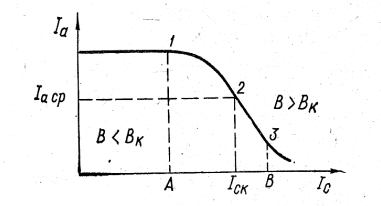
\includegraphics[width = 0.5\textwidth]{image/image1.png}
    \caption{Рис. 1}
    \label{fig:image1}
\end{figure}


\begin{figure}[!h]
    \centering
    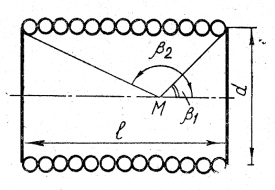
\includegraphics[width = 0.5\textwidth]{image/image2.png}
    \caption{Рис. 2}
    \label{fig:image2}
\end{figure}


Если диод расположен так, что анод и катод находятся в средней части соленоида, то $\beta _2 = 180^o - \beta _1$, $\cos{\beta _2} = -\cos{\beta _1}$, и формула (\ref{eq:formula3}) принимает вид

$B = \mu _0 I_c n_0 \cos{\beta _1}$.

Так как 

$\cos{\beta _1} = \frac{\frac{l}{2}}{\sqrt[2]{(\frac{l}{2})^2 + (\frac{d}{2})^2}} = \frac{l}{\sqrt[2]{l^2 + d^2}}$,

$B = \mu _0 I_c n_0 \frac{l}{\sqrt[2]{l^2 + d^2}}$,

где $l$ "--- длина соленоида, $d$ "--- средний диаметр его витков.

Величина критической индукции магнитного поля определяется соотношением

\begin{equation}
    B_k = \mu _0 I_ck n_0 \frac{l}{\sqrt[2]{l^2 + d^2}}
    \label{eq:formula4}
\end{equation}
